\chapter{Materiais inorgânicos e nanomateriais}\label{ch:b3:inorganic-materials}

Uma placa de \omterm{def:b3:inorganic-materials:sol-gel}{aerogel} de sílica, um sólido que é quase todo ar, sustenta uma flor acima de uma
chama de gás sem deixá-la murchar. É um vidro, feito não pela fusão de areia, mas
deixando um líquido endurecer em um \omterm{def:b3:colloids:colloid}{gel} e secando depois o \omterm{def:b3:colloids:colloid}{gel} sem deixá-lo
colapsar. A química dos materiais trabalha nessa ordem: escolher a estrutura, depois
a rota que a produz, depois ler as propriedades. Este capítulo segue
as rotas para os sólidos inorgânicos, as estruturas das \omterm{def:b3:inorganic-materials:ceramic}{cerâmicas}, dos vidros e dos cristais
porosos, e o que acontece com a matéria quando uma partícula mede apenas alguns nanômetros
de diâmetro.

\begin{recall}
O volume do 1.º ano descreveu os tipos de estrutura cristalina, os sítios intersticiais,
os alótropos, o grafite e o diamante; o volume do 2.º ano, os diagramas de fases, a temperatura
de transição vítrea e os polímeros. O \cref{ch:b3:surfaces-catalysis} definiu a
\omterm{def:b3:surfaces-catalysis:surface-area}{área superficial específica}, o \cref{ch:b3:colloids}, os \omterm{def:b3:colloids:colloid}{sóis} e os géis,
o \cref{ch:b3:solid-state}, as bandas, os \omterm{def:b3:solid-state:defects}{defeitos pontuais} e os \omterm{def:b3:solid-state:ionic-conductor}{condutores iônicos};
o \cref{ch:b3:quantum-model-systems} resolveu a \omterm{def:b3:quantum-model-systems:box}{partícula na caixa}, e o
\cref{ch:b3:point-groups} deu o grupo icosaédrico.
\end{recall}

\begin{omfigure}
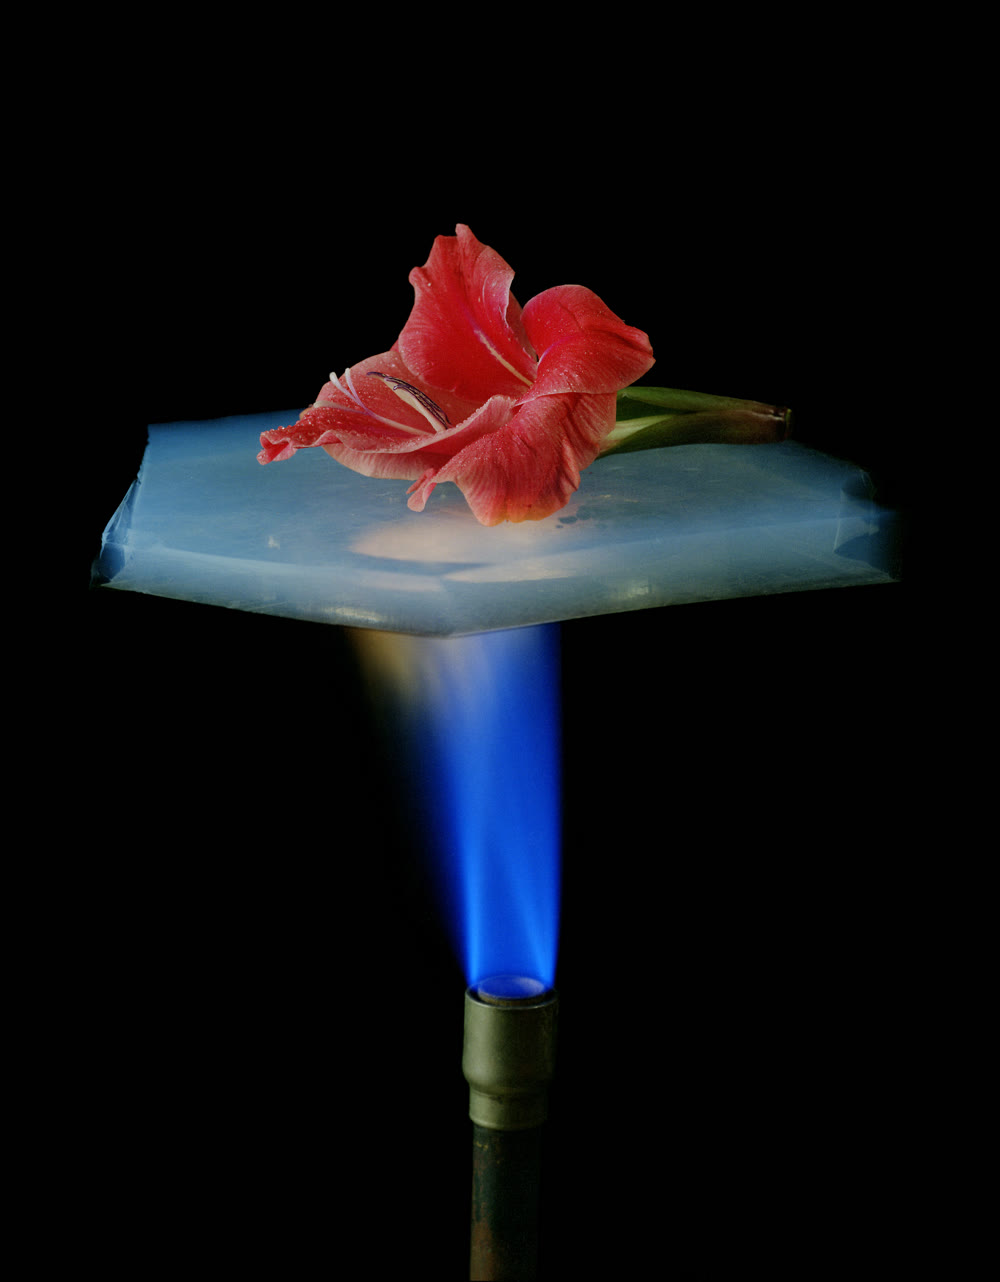
\includegraphics[width=0.38\linewidth]{images/book4/aerogel-flower.jpg}

{\small Uma flor sobre uma placa de \omterm{def:b3:inorganic-materials:sol-gel}{aerogel} de sílica acima de uma chama de gás: o \omterm{def:b3:inorganic-materials:sol-gel}{aerogel}, um
\omterm{def:b3:colloids:colloid}{gel} seco que é quase todo espaço vazio, conduz muito mal o calor. Fotografia:
NASA/JPL, domínio público.}
\end{omfigure}

\section{Rotas de síntese}

\begin{definition}[Método cerâmico]\label{def:b3:inorganic-materials:ceramic-method}
O \emph{método cerâmico}\index{metodo ceramico@método cerâmico} prepara um composto sólido
moendo juntos os reagentes sólidos e aquecendo-os, muitas vezes durante dias e
com novas moagens, a temperaturas altas o bastante para que os íons se difundam através dos
sólidos.
\end{definition}

A reação entre dois sólidos ocorre em seu contato, e o produto forma uma
camada entre eles que os íons precisam então atravessar: a etapa mais lenta
é a difusão, e ela se torna mais lenta à medida que a camada se espessa.

\begin{proposition}[Crescimento parabólico]\label{prop:b3:inorganic-materials:parabolic}
Se o crescimento de uma camada de produto é limitado pela difusão através dela, sua
espessura cresce como $x^2 = kt$.
\end{proposition}

\begin{proof}
Com concentrações fixas nas duas faces da camada, o fluxo através dela
segue a lei de Fick, $J = D\Delta c/x$. A camada cresce proporcionalmente ao fluxo:
$\dd x/\dd t = \lambda J = \lambda D\Delta c/x$, com $\lambda$ o volume de produto por mol transportado. Então
$x\,\dd x = \lambda D\Delta c\,\dd t$, e integrando a partir de $x = 0$ em $t = 0$ obtém-se $x^2 = 2\lambda D\Delta c\,t = kt$.
\end{proof}

Dobrar o tamanho das partículas multiplica, assim, o tempo de reação por quatro: daí
a moagem fina, a mistura em escala atômica em um precursor (um oxalato misto ou um
\omterm{def:b3:colloids:colloid}{gel} de citrato que se decompõe no produto desejado) ou uma rota em solução.

\begin{definition}[Processo sol--gel]\label{def:b3:inorganic-materials:sol-gel}
O \emph{processo sol--gel}\index{processo sol--gel} prepara um óxido por
hidrólise e condensação de precursores moleculares, em geral alcóxidos, em
solução: a solução se torna um \omterm{def:b3:colloids:colloid}{sol} de pequenos aglomerados de óxido, depois um \omterm{def:b3:colloids:colloid}{gel}, uma
rede sólida contínua preenchida de líquido. Seco por evaporação, o \omterm{def:b3:colloids:colloid}{gel}
se contrai em um \emph{xerogel}\index{xerogel} denso; seco acima do ponto
crítico do líquido, o que o remove sem interface líquido--gás, ele conserva
seu volume como um \emph{aerogel}\index{aerogel}.
\end{definition}

\begin{omfigure}
\setchemfig{atom sep=2.0em}
\schemestart
\chemfig{RO-Si(-[2]OR)(-[6]OR)-OR}
\+ \chemfig{H_2O}
\arrow{->[hidrólise]}[,1.4]
\chemfig{RO-Si(-[2]OR)(-[6]OR)-OH}
\+ ROH
\schemestop
\par\bigskip
\schemestart
\chemfig{{\equiv}Si-OH}
\+
\chemfig{HO-Si{\equiv}}
\arrow{->[condensação]}[,1.6]
\chemfig{{\equiv}Si-O-Si{\equiv}}
\+ \chemfig{H_2O}
\schemestop
\par\medskip

{\small Química sol--gel de um alcóxido de silício (R: um grupo alquila, etila no
ortossilicato de tetraetila): a água substitui grupos alcóxi por grupos hidróxi, e
dois silanóis se condensam em uma ponte siloxano. Repetidas, as condensações constroem
uma rede tridimensional de sílica.}
\end{omfigure}

As duas reações juntas dão, para reação completa,
$\ce{Si(OC2H5)4 + 2H2O -> SiO2 + 4C2H5OH}$. A catálise ácida torna a hidrólise rápida e a
condensação lenta, dando polímeros finos, em forma de cadeia; a catálise básica, o
contrário, dando partículas densas. Os revestimentos (camadas antirreflexo sobre vidro)
são feitos mergulhando uma peça no \omterm{def:b3:colloids:colloid}{sol} e retirando-a.

\begin{definition}[Síntese hidrotérmica]\label{def:b3:inorganic-materials:hydrothermal}
A \emph{síntese hidrotérmica}\index{sintese hidrotermica@síntese hidrotérmica} cristaliza um
sólido a partir de água acima de seu ponto de ebulição normal, em recipiente fechado, sob sua
própria pressão de vapor; a \emph{síntese solvotérmica}\index{sintese solvotermica@síntese solvotérmica}
faz o mesmo em outro solvente.
\end{definition}

\begin{definition}[Deposição química em fase vapor]\label{def:b3:inorganic-materials:cvd}
A \emph{deposição química em fase vapor}\index{deposicao quimica em fase vapor@deposição química em fase vapor} (CVD) faz crescer um
filme sólido sobre uma superfície aquecida pela reação ali de precursores gasosos, como o
silício a partir do silano, $\ce{SiH4 -> Si + 2H2}$, ou o diamante a partir de metano e hidrogênio.
\end{definition}

\begin{method}[Escolher uma rota de síntese]\label{met:b3:inorganic-materials:route}
\begin{enumerate}
  \item Um óxido estável e refratário em pó maciço: o \omterm{def:b3:inorganic-materials:ceramic-method}{método cerâmico}, com um
        precursor se a mistura for difícil.
  \item Uma fase metaestável, um pó fino ou um revestimento a baixa temperatura:
        sol--gel ou uma precipitação.
  \item Grandes monocristais de uma fase solúvel apenas em água quente (quartzo) ou
        uma estrutura construída em torno de um molde (\omterm{def:b3:inorganic-materials:zeolite}{zeólitas}): hidrotérmica.
  \item Um filme fino e puro sobre um substrato (camadas semicondutoras): CVD.
\end{enumerate}
\end{method}

\begin{inthelab}[Um revestimento sol--gel e uma autoclave]
O ortossilicato de tetraetila é agitado com etanol, água e uma gota de ácido
até a solução ficar límpida; uma lâmina de vidro limpa é mergulhada e retirada a
velocidade lenta e constante, seca e aquecida, deixando um filme de sílica fino o bastante para
mostrar cores de interferência. Para uma \omterm{def:b3:inorganic-materials:hydrothermal}{síntese hidrotérmica}, os reagentes são colocados
em um revestimento interno de politetrafluoroetileno, preenchido no máximo até cerca de dois terços para
que o líquido em expansão não encha o recipiente, fechados em uma autoclave de aço
e aquecidos em estufa; a autoclave só é aberta depois de fria.
\end{inthelab}

\begin{omfigure}
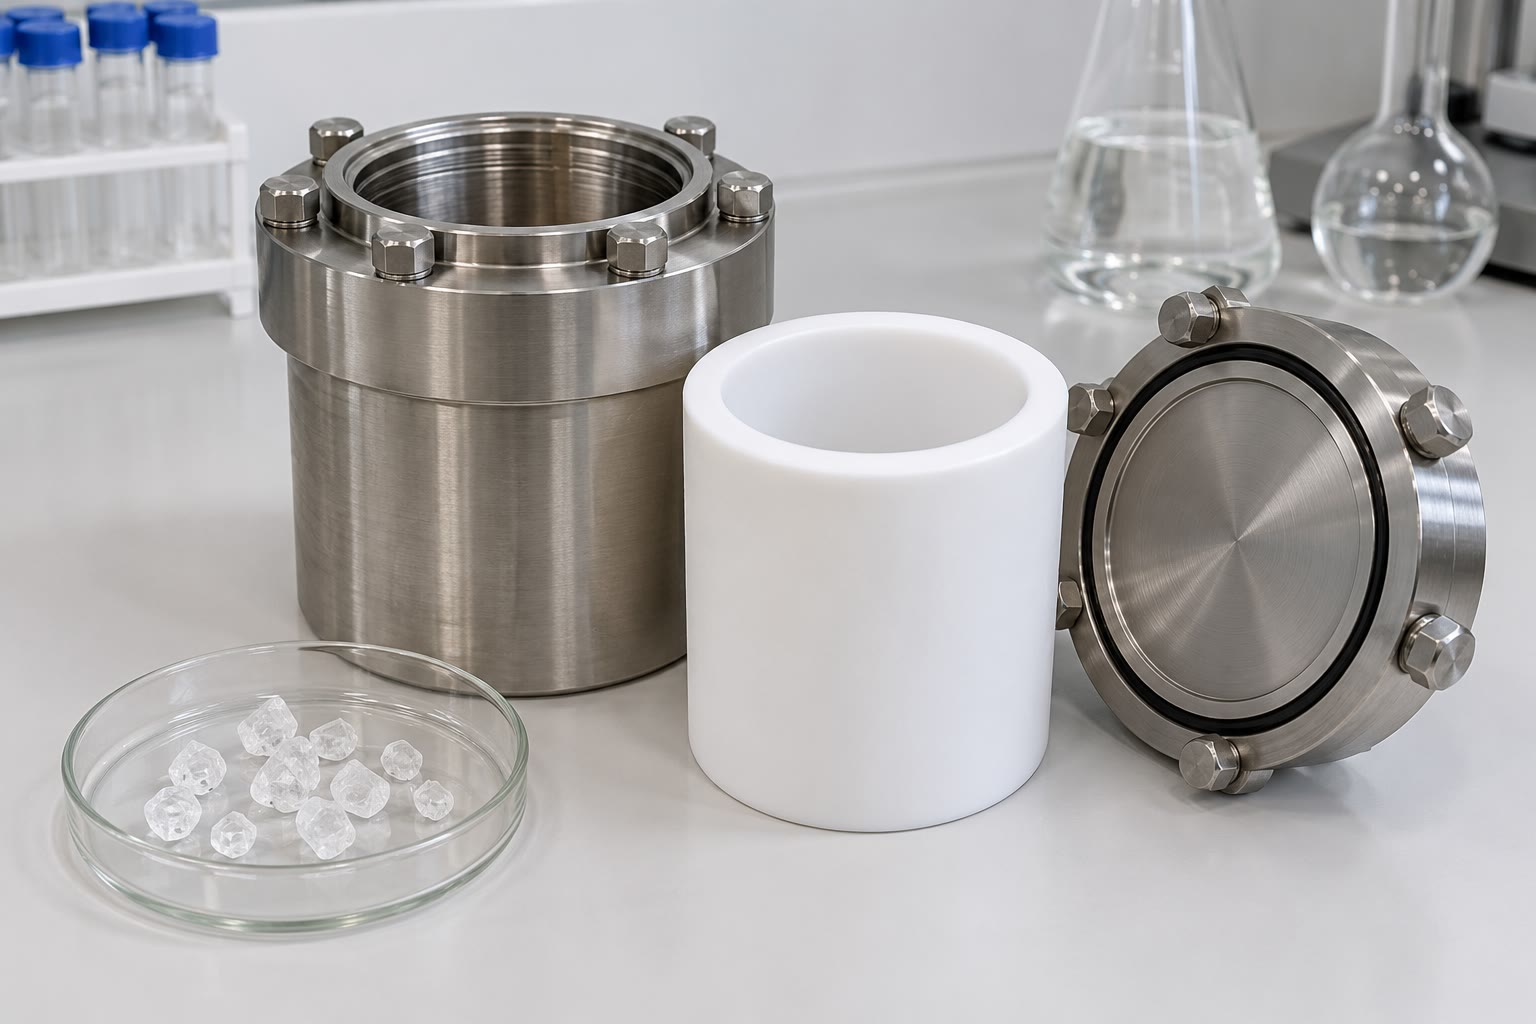
\includegraphics[width=0.5\linewidth]{images/book4/ai/b3-23-autoclave.jpg}

{\small Uma autoclave de laboratório para \omterm{def:b3:inorganic-materials:hydrothermal}{síntese hidrotérmica}: um corpo de aço com uma
tampa aparafusada, um revestimento interno de polímero branco que contém a mistura reacional, e cristais
crescidos nela.}
\end{omfigure}

\section{Cerâmicas e vidros}

\begin{definition}[Cerâmica]\label{def:b3:inorganic-materials:ceramic}
Uma \emph{cerâmica}\index{ceramica@cerâmica} é um sólido inorgânico não metálico preparado
pelo aquecimento de um pó: óxidos, nitretos e carbetos, ou produtos de argila.
\end{definition}

\begin{definition}[Estrutura perovskita]\label{def:b3:inorganic-materials:perovskite}
A \emph{estrutura perovskita}\index{estrutura perovskita} de um óxido $\mathrm{ABO_3}$
tem os cátions B pequenos nos centros de octaedros $\mathrm{BO_6}$ que compartilham vértices e
os cátions A grandes nas cavidades de coordenação doze entre eles; na
cela cúbica ideal, B fica no centro, O nos centros das faces, A nos vértices.
O \emph{fator de tolerância}\index{fator de tolerancia@fator de tolerância} mede quão bem os íons
se encaixam:
\[
  t = \frac{r_A + r_O}{\sqrt2\,(r_B + r_O)}.
\]
\end{definition}

\begin{omfigure}
\tdplotsetmaincoords{60}{100}
\begin{tikzpicture}[tdplot_main_coords, scale=1.5, font=\small,
  aA/.style={om atom, ball color=green!45!black, minimum size=7.4mm},
  aB/.style={om atom, ball color=black!35, minimum size=4.4mm},
  aOs/.style={om atom, ball color=red!80, minimum size=4.8mm}]
  \pic[transform shape] {omcubeo={2}};
  % atoms back to front for view 60/100 (depth 0.853x + 0.150y + 0.5z)
  \node[aA] at (0,0,0) {};
  \node[aA] at (0,2,0) {};
  \node[aOs] (o1) at (0,1,1) {};
  \node[aA] at (0,0,2) {};
  \node[aOs] (o2) at (1,1,0) {};
  \node[aA] at (0,2,2) {};
  \node[aOs] (o3) at (1,0,1) {};
  \node[aB] (b) at (1,1,1) {};
  \node[aOs] (o4) at (1,2,1) {};
  \node[aA] at (2,0,0) {};
  \node[aOs] (o5) at (1,1,2) {};
  \node[aA] at (2,2,0) {};
  \node[aOs] (o6) at (2,1,1) {};
  \node[aA] at (2,0,2) {};
  \node[aA] at (2,2,2) {};
  \begin{scope}[on background layer]
    \draw[omMeth!70, line width=0.6pt] (o1.center) -- (o2.center) -- (o6.center) -- (o5.center) -- cycle
      (o3.center) -- (o2.center) -- (o4.center) -- (o5.center) -- cycle
      (o1.center) -- (o3.center) -- (o6.center) -- (o4.center) -- cycle;
    \draw[bond] (b.center) -- (o1.center) (b.center) -- (o2.center) (b.center) -- (o3.center)
      (b.center) -- (o4.center) (b.center) -- (o5.center) (b.center) -- (o6.center);
  \end{scope}
  \node[anchor=west] at (2,3.35,2) {A};
  \node[anchor=west] at (2,3.35,1) {O};
  \node[anchor=west] at (2,3.35,0) {B};
  \node[aA, minimum size=4mm] at (2,3.2,2) {};
  \node[aOs, minimum size=3.2mm] at (2,3.2,1) {};
  \node[aB, minimum size=3mm] at (2,3.2,0) {};
\end{tikzpicture}

{\small A cela cúbica de perovskita $\mathrm{ABO_3}$: um cátion B (cinza) no centro de um
octaedro de seis íons óxido nos centros das faces (arestas verdes), os cátions A
nos vértices. Cada íon A de vértice é compartilhado por oito celas e cada oxigênio por
duas: um A, um B e três O por cela.}
\end{omfigure}

\begin{proposition}[Fator de tolerância ideal]\label{prop:b3:inorganic-materials:tolerance}
Na perovskita cúbica ideal, com os íons em contato ao longo das direções B--O e A--O,
$t = 1$.
\end{proposition}

\begin{proof}
Com aresta $a$, B no centro e O no centro de uma face estão a $a/2$ um do outro: $r_B + r_O = a/2$.
A em um vértice e O no centro de uma face adjacente estão a meia diagonal de face
um do outro: $r_A + r_O = a\sqrt2/2$. Dividindo, $(r_A + r_O)/(r_B + r_O) = \sqrt2$, logo $t = 1$.
\end{proof}

Quando $t$ é um pouco menor que 1, o íon A é pequeno demais para sua cavidade e os
octaedros se inclinam para se fechar em torno dele, abaixando a simetria; quando $t$ é maior que 1,
o íon B é pequeno demais para seu octaedro e pode sair do centro.

\begin{definition}[Ferroelétrico]\label{def:b3:inorganic-materials:ferroelectric}
Um \emph{ferroelétrico}\index{ferroeletrico@ferroelétrico} é um cristal com uma polarização
elétrica espontânea que um campo elétrico aplicado pode inverter.
\end{definition}

% ledger: rion:Ba2+XII, rion:Ti4+VI, rion:O2-VI
O titanato de bário é o caso clássico: com $r(\ce{Ba^2+}) = \qty{161}{pm}$ (coordenação doze),
$r(\ce{Ti^4+}) = \qty{60.5}{pm}$ e $r(\ce{O^2-}) = \qty{140}{pm}$, $t = 1.06$. Abaixo de uma temperatura de transição, os
íons titânio se deslocam do centro, todos no mesmo sentido dentro de um domínio,
e o cristal se polariza; a enorme permissividade perto da transição faz do
titanato de bário o dielétrico da maioria dos capacitores cerâmicos.

\begin{definition}[Vidros de óxidos]\label{def:b3:inorganic-materials:glass}
Um \emph{vidro de óxidos}\index{vidro de oxidos@vidro de óxidos} é um sólido amorfo de óxidos, obtido por
resfriamento de um material fundido sem cristalização. Seus \emph{formadores de
rede}\index{formador de rede} ($\ce{SiO2}$, $\ce{B2O3}$, $\ce{P2O5}$) constroem uma rede contínua de
poliedros que compartilham vértices; seus \emph{modificadores de rede}\index{modificador de rede}
($\ce{Na2O}$, $\ce{CaO}$) rompem pontes nessa rede, cada íon óxido adicionado transformando um
oxigênio em ponte em dois oxigênios não ligados em ponte, com os cátions alojados nos
vazios.
\end{definition}

\begin{omfigure}
\begin{tikzpicture}
\begin{axis}[name=c, width=0.5\linewidth, axis equal image, hide axis, xmin=-1.2, xmax=12.6, ymin=-1.2, ymax=8.7]
\addplot[quiver={u=\thisrow{u}, v=\thisrow{v}}, -, black!60, line width=0.6pt] table {figdata/out/bachelor-3-glass-network-crystal-bonds.dat};
\addplot[only marks, mark=*, mark size=2.2pt, omDef] table {figdata/out/bachelor-3-glass-network-crystal-T.dat};
\addplot[only marks, mark=*, mark size=1.3pt, omThm, mark options={fill=white}] table {figdata/out/bachelor-3-glass-network-crystal-O.dat};
\end{axis}
\begin{axis}[at={(c.east)}, anchor=west, xshift=0.2cm, width=0.5\linewidth, axis equal image, hide axis, xmin=-1.2, xmax=12.6, ymin=-1.2, ymax=8.7]
\addplot[quiver={u=\thisrow{u}, v=\thisrow{v}}, -, black!60, line width=0.6pt] table {figdata/out/bachelor-3-glass-network-glass-bonds.dat};
\addplot[only marks, mark=*, mark size=2.2pt, omDef] table {figdata/out/bachelor-3-glass-network-glass-T.dat};
\addplot[only marks, mark=*, mark size=1.3pt, omThm, mark options={fill=white}] table {figdata/out/bachelor-3-glass-network-glass-O.dat};
\addplot[only marks, mark=*, mark size=1.5pt, omThm] table {figdata/out/bachelor-3-glass-network-glass-NBO.dat};
\addplot[only marks, mark=*, mark size=2.6pt, omProp] table {figdata/out/bachelor-3-glass-network-glass-Na.dat};
\end{axis}
\end{tikzpicture}

{\small Uma imagem bidimensional de um cristal e de um vidro de mesma
composição (azul: formadores tricoordenados; círculos vermelhos vazados: oxigênios
em ponte). À esquerda, o cristal repete um único anel. À direita, o vidro: cada formador
ainda tem três oxigênios a distâncias quase iguais, mas os anéis têm cinco,
seis ou sete membros e nada se repete; em dois lugares, um modificador rompeu uma
ponte, deixando dois oxigênios não ligados em ponte (vermelho cheio) e um cátion (laranja) no
vazio. Rede-modelo, relaxada com molas.}
\end{omfigure}

William Zachariasen argumentou em 1932 que um óxido forma facilmente um vidro quando seu
cátion é cercado por poucos oxigênios (três ou quatro), cada oxigênio liga no máximo
dois cátions e os poliedros compartilham vértices, e não arestas ou faces: então uma
rede aleatória custa pouco mais energia que o cristal. O vidro de janela é
sílica com óxidos de sódio e de cálcio como modificadores, que abaixam a temperatura
de fusão. O vidro temperado das telas de celular é imerso em nitrato de potássio
fundido: íons $\ce{K+}$, maiores, substituem os íons $\ce{Na+}$ da superfície e, apertados,
a põem sob compressão, de modo que as trincas não se abrem.

\section{Sólidos porosos: zeólitas e redes}

\begin{definition}[Zeólitas]\label{def:b3:inorganic-materials:zeolite}
Uma \emph{zeólita}\index{zeolita@zeólita} é um aluminossilicato cristalino cuja
estrutura de tetraedros $\ce{SiO4}$ e $\ce{AlO4}$ que compartilham vértices delimita cavidades e
canais de tamanho molecular, com cátions trocáveis e água em seu interior. Uma
\emph{peneira molecular}\index{peneira molecular} é um sólido poroso que admite
moléculas de acordo com seu tamanho; a \emph{seletividade de forma}\index{seletividade de forma}
é o controle de uma reação pelo tamanho e pela forma dos poros nos
quais ela ocorre.
\end{definition}

Cada tetraedro $\ce{AlO4}$ carrega uma carga negativa a mais que um $\ce{SiO4}$
(alumínio(III) no lugar de silício(IV)); os cátions nas cavidades, $\ce{Na+}$ ou $\ce{Ca^2+}$,
a compensam e podem ser trocados.

\begin{proposition}[Regra de Löwenstein]\label{prop:b3:inorganic-materials:lowenstein}
Em uma estrutura de \omterm{def:b3:inorganic-materials:zeolite}{zeólita}, dois tetraedros $\ce{AlO4}$ nunca compartilham um oxigênio: as ligações Al--O--Al
estão ausentes (uma observação feita sobre todas as estruturas de aluminossilicatos conhecidas). Em
consequência, a razão Si/Al de uma \omterm{def:b3:inorganic-materials:zeolite}{zeólita} é pelo menos 1.
\end{proposition}

\begin{proof}[Demonstração da consequência]
Cada alumínio tem quatro oxigênios, cada um compartilhado com um silício pela regra:
$4N_{\mathrm{Al}}$ ligações Al--O--Si. Cada silício tem apenas quatro oxigênios, de modo que participa de
no máximo quatro dessas ligações: $4N_{\mathrm{Al}} \le 4N_{\mathrm{Si}}$, isto é, $N_{\mathrm{Si}}/N_{\mathrm{Al}} \ge 1$. A igualdade obriga todo
silício a ter quatro vizinhos alumínio: Si e Al se alternam.
\end{proof}

\begin{omfigure}
\tdplotsetmaincoords{55}{135}
\begin{tikzpicture}[tdplot_main_coords, scale=0.85, font=\small, baseline=(current bounding box.center),
  tSi/.style={circle, inner sep=0pt, minimum size=2.6mm, draw=black!70, fill=omDef!80},
  tAl/.style={circle, inner sep=0pt, minimum size=2.6mm, draw=black!70, fill=omProp!80}]
  % edges of a truncated octahedron (vertices: permutations of (0, +-1, +-2));
  % hidden edges (both faces facing away for this view) dashed
  \foreach \a/\b/\c/\d/\e/\f in {-2/-1/0/-2/0/-1, -2/-1/0/-2/0/1, -2/-1/0/-1/-2/0, -2/0/-1/-2/1/0, -2/0/-1/-1/0/-2, -1/-2/0/0/-2/-1, -1/-2/0/0/-2/1, -1/0/-2/0/-1/-2, -1/0/-2/0/1/-2, 0/-2/-1/0/-1/-2, 0/-2/-1/1/-2/0, 0/-1/-2/1/0/-2}
    \draw[black!40, dashed] (\a,\b,\c) -- (\d,\e,\f);
  \foreach \a/\b/\c/\d/\e/\f in {-2/0/1/-2/1/0, -2/0/1/-1/0/2, -2/1/0/-1/2/0, -1/0/2/0/-1/2, -1/0/2/0/1/2, -1/2/0/0/2/-1, -1/2/0/0/2/1, 0/-2/1/0/-1/2, 0/-2/1/1/-2/0, 0/-1/2/1/0/2, 0/1/-2/0/2/-1, 0/1/-2/1/0/-2, 0/1/2/0/2/1, 0/1/2/1/0/2, 0/2/-1/1/2/0, 0/2/1/1/2/0, 1/-2/0/2/-1/0, 1/0/-2/2/0/-1, 1/0/2/2/0/1, 1/2/0/2/1/0, 2/-1/0/2/0/-1, 2/-1/0/2/0/1, 2/0/-1/2/1/0, 2/0/1/2/1/0}
    \draw[black!75, line width=0.7pt] (\a,\b,\c) -- (\d,\e,\f);
  % T atoms back to front; hidden ones paler
  \foreach \x/\y/\z/\k/\v in {-2/-1/0/Si/0, -1/-2/0/Al/0, -2/0/-1/Al/0, 0/-2/-1/Si/0, -1/0/-2/Si/0, 0/-1/-2/Al/0, -2/0/1/Al/1, 0/-2/1/Si/1, -2/1/0/Si/1, 1/-2/0/Al/1, 0/1/-2/Al/1, 1/0/-2/Si/1, -1/0/2/Si/1, 0/-1/2/Al/1, -1/2/0/Al/1, 2/-1/0/Si/1, 0/2/-1/Si/1, 2/0/-1/Al/1, 0/1/2/Al/1, 1/0/2/Si/1, 0/2/1/Si/1, 2/0/1/Al/1, 1/2/0/Al/1, 2/1/0/Si/1}
    \node[t\k, opacity=0.35+0.65*\v] at (\x,\y,\z) {};
\end{tikzpicture}
\hspace{1.2cm}
\begin{tikzpicture}[font=\small, scale=0.8, baseline=(current bounding box.center)]
  \foreach \i in {0,1,2} \foreach \j in {0,1,2} {
    \fill[omDef!70] ($(2.2*\i,2.2*\j)+(-0.28,-0.28)$) rectangle +(0.56,0.56);
  }
  \foreach \i in {0,1} \foreach \j in {0,1,2} {
    \draw[black!70, line width=0.8pt] (2.2*\i+0.28,2.2*\j) -- (2.2*\i+0.75,2.2*\j);
    \draw[black!70, line width=0.8pt] (2.2*\i+1.45,2.2*\j) -- (2.2*\i+1.92,2.2*\j);
    \node[draw=black!70, regular polygon, regular polygon sides=6, minimum size=5.6mm, inner sep=0pt] at (2.2*\i+1.1,2.2*\j) {};
  }
  \foreach \i in {0,1,2} \foreach \j in {0,1} {
    \draw[black!70, line width=0.8pt] (2.2*\i,2.2*\j+0.28) -- (2.2*\i,2.2*\j+0.75);
    \draw[black!70, line width=0.8pt] (2.2*\i,2.2*\j+1.45) -- (2.2*\i,2.2*\j+1.92);
    \node[draw=black!70, regular polygon, regular polygon sides=6, minimum size=5.6mm, inner sep=0pt] at (2.2*\i,2.2*\j+1.1) {};
  }
  \node[font=\scriptsize, align=center] at (1.1,-0.85) {nó $\ce{Zn4O}$ $+$ ligante tereftalato};
\end{tikzpicture}

{\small À esquerda: uma cavidade sodalita, a unidade de construção da \omterm{def:b3:inorganic-materials:zeolite}{zeólita} A, com um
átomo tetraédrico em cada vértice (os oxigênios, no meio de cada aresta, não são
desenhados); silício (azul) e alumínio (laranja) se alternam, como exige a regra de
Löwenstein quando Si/Al = 1. À direita: uma camada de uma \omterm{def:b3:inorganic-materials:mof}{rede metalorgânica},
esquemática: aglomerados $\ce{Zn4O}$ (quadrados) unidos por ligantes benzeno-1,4-dicarboxilato
(anéis) em uma grade cúbica de poros grandes.}
\end{omfigure}

\begin{method}[Fórmula e capacidade de troca de uma zeólita]\label{met:b3:inorganic-materials:zeolite-formula}
\begin{enumerate}
  \item Escreva a estrutura como $\mathrm{[(AlO_2)_x(SiO_2)_y]^{x-}}$: Si/Al $= y/x$.
  \item A carga $-x$ da estrutura é compensada por cátions: $x$ monovalentes ou $x/2$
        divalentes.
  \item A capacidade de troca é a quantidade de carga trocável por grama:
        $x/M$ mols de cátions monovalentes, $x/2M$ de divalentes, com $M$ a
        massa molar da fórmula tal como pesada (anidra ou hidratada).
\end{enumerate}
\end{method}

\begin{proposition}[Capacidade de troca]\label{prop:b3:inorganic-materials:exchange-capacity}
A capacidade de uma \omterm{def:b3:inorganic-materials:zeolite}{zeólita} para um cátion de carga $z$ é de $x/(zM)$ mols por grama,
onde $x$ é o número de átomos de alumínio em uma fórmula de massa molar $M$.
\end{proposition}

\begin{proof}
Cada alumínio contribui com uma carga negativa para a estrutura; a
eletroneutralidade exige $x$ unidades de carga positiva, todas trocáveis, logo
$x/z$ cátions de carga $z$ por unidade de fórmula, isto é, por massa $M$.
\end{proof}

% ledger: iza:LTA.window, iza:MFI.channels
A \omterm{def:b3:inorganic-materials:zeolite}{zeólita} A tem janelas de oito tetraedros, de \qty{0.41}{nm}: a água e os íons
pequenos passam, as moléculas ramificadas não. A ZSM-5 tem dois conjuntos de canais de dez
tetraedros, de cerca de 0.51 a \qty{0.56}{nm}: na conversão do metanol ou na
alquilação do tolueno, o esguio \textit{para}-xileno se difunde para fora muito mais depressa que
seus isômeros \textit{orto} e \textit{meta}, que ficam e se isomerizam. Isso é a \omterm{def:b3:inorganic-materials:zeolite}{seletividade
de forma}.

\begin{definition}[Redes metalorgânicas]\label{def:b3:inorganic-materials:mof}
Uma \emph{rede metalorgânica}\index{rede metalorganica@rede metalorgânica} (MOF) é um
sólido cristalino construído a partir de íons ou aglomerados metálicos unidos por ligantes
orgânicos politópicos em uma rede porosa. Uma \emph{unidade de construção
secundária}\index{unidade de construcao secundaria@unidade de construção secundária} é o aglomerado metálico com seus
grupos coordenantes, tratado como um nó da rede; a \emph{síntese
reticular}\index{sintese reticular@síntese reticular} é o planejamento de uma estrutura pela escolha de
nós e ligantes de geometria dada, de modo que eles se montem em uma rede escolhida.
\end{definition}

% ledger: cod:MOF5.formula, cod:MOF5.a
No MOF-5, aglomerados $\ce{Zn4O}$ com seis grupos carboxilato são nós octaédricos,
e ligantes benzeno-1,4-dicarboxilato os unem ao longo das arestas de uma rede
cúbica, $a = \qty{25.82}{\angstrom}$ para uma cela de oito nós. Substituir o ligante por um mais
longo conserva a rede e aumenta os poros: essa é a ideia reticular. Essas
redes têm áreas superficiais de milhares de metros quadrados por grama e são
estudadas para armazenar hidrogênio e metano e para capturar dióxido de carbono.

\begin{definition}[Tamanhos de poro]\label{def:b3:inorganic-materials:pores}
% ledger: pore:micro, pore:macro
Por convenção, os \emph{microporos}\index{microporo} têm menos de \qty{2}{nm},
os \emph{mesoporos}\index{mesoporo} entre 2 e \qty{50}{nm}, e
os \emph{macroporos}\index{macroporo} mais de \qty{50}{nm}.
\end{definition}

As \omterm{def:b3:inorganic-materials:zeolite}{zeólitas} e a maioria dos MOFs são microporosos; os géis de sílica e os aerogéis, mesoporosos.

\section{Nanopartículas}

\begin{definition}[Nanomateriais]\label{def:b3:inorganic-materials:nano}
Um \emph{nanomaterial}\index{nanomaterial} tem pelo menos uma dimensão entre
cerca de 1 e \qty{100}{nm}; uma \emph{nanopartícula}\index{nanoparticula@nanopartícula} tem as
três.
\end{definition}

\begin{proposition}[Aglomerados mágicos]\label{prop:b3:inorganic-materials:magic}
Um aglomerado cuboctaédrico formado por um átomo central e $n$ camadas completas tem
\[
  N(n) = \frac{10n^3 + 15n^2 + 11n + 3}{3}
\]
átomos, dos quais $10n^2 + 2$ estão na superfície: 13, 55, 147, 309, \dots
\end{proposition}

\begin{proof}
A $k$-ésima camada de um cuboctaedro tem 12 vértices, 24 arestas com $k - 1$ átomos
no interior de cada uma, 8 faces triangulares com $(k - 1)(k - 2)/2$ átomos internos cada e 6
faces quadradas com $(k - 1)^2$: no total, $12 + 24(k - 1) + 4(k - 1)(k - 2) + 6(k - 1)^2 = 10k^2 + 2$. Então
$N(n) = 1 + \sum_{k=1}^{n}(10k^2 + 2) = 1 + \frac{10n(n + 1)(2n + 1)}{6} + 2n$, que, desenvolvida, dá a fórmula; a
camada externa, de $10n^2 + 2$ átomos, é a superfície.
\end{proof}

\begin{omfigure}
\begin{tikzpicture}
\begin{axis}[name=a, width=0.47\linewidth, height=5.4cm, xmin=0, xmax=18, ymin=0, ymax=1,
  axis lines=left, xlabel={diâmetro / \unit{nm}}, ylabel={fração de átomos na superfície},
  tick label style={font=\scriptsize}, label style={font=\small}]
\addplot[omDef, thick, mark=*, mark size=1pt] table[x=diam_nm, y=fsurf] {figdata/out/bachelor-3-nanoparticle-size.dat};
\end{axis}
\begin{axis}[at={(a.east)}, anchor=west, xshift=1.5cm, width=0.47\linewidth, height=5.4cm,
  xmin=0.8, xmax=6, ymin=0, ymax=3, axis lines=left,
  xlabel={raio $R$ / \unit{nm}}, ylabel={energia de confinamento / \unit{eV}},
  tick label style={font=\scriptsize}, label style={font=\small}]
\addplot[omThm, thick] table[x=R_nm, y=dE_eV] {figdata/out/bachelor-3-nanoparticle-size-b.dat};
\end{axis}
\end{tikzpicture}

{\small À esquerda: fração de átomos na superfície de aglomerados cuboctaédricos de ouro
em função de seu diâmetro: mais da metade para aglomerados menores que cerca de
\qty{3}{nm}, ainda um quinto a \qty{8}{nm}. À direita: energia de confinamento de um
par elétron--buraco em um \omterm{def:b3:inorganic-materials:quantum-dot}{ponto quântico} esférico (\omterm{def:b3:quantum-model-systems:oscillator}{massa reduzida} do modelo $0.10\,m_e$),
que se soma à \omterm{def:b3:solid-state:band}{banda proibida} e cai como $1/R^2$.}
\end{omfigure}

Com uma grande fração de seus átomos na superfície, onde têm menos
vizinhos, uma \omterm{def:b3:inorganic-materials:nano}{nanopartícula} funde a uma temperatura mais baixa que o metal maciço,
é mais reativa e pode ser um catalisador muito melhor: o ouro maciço é inerte, partículas de
ouro de alguns nanômetros oxidam o monóxido de carbono à temperatura ambiente.

\begin{definition}[Pontos quânticos]\label{def:b3:inorganic-materials:quantum-dot}
Um \emph{ponto quântico}\index{ponto quantico@ponto quântico} é um nanocristal \omterm{def:b3:solid-state:classes}{semicondutor} pequeno
o bastante para que o confinamento de seus elétrons e \omterm{def:b3:solid-state:carriers}{buracos} eleve sua \omterm{def:b3:solid-state:band}{banda proibida}
acima da do sólido maciço.
\end{definition}

\begin{theorem}[Confinamento em uma esfera]\label{thm:b3:inorganic-materials:quantum-dot}
Uma partícula de massa $m$ confinada em uma esfera de raio $R$ por paredes infinitas tem
a energia do estado fundamental $E = \hbar^2\pi^2/(2mR^2) = h^2/(8mR^2)$, com função de onda $\psi \propto \sin(\pi r/R)/r$.
\end{theorem}

\begin{proof}
Para um estado de simetria esférica $\psi(r) = u(r)/r$, o laplaciano dá
$\nabla^2\psi = u''/r$, de modo que a \omterm{thm:b3:quantum-model-systems:schrodinger}{equação de Schrödinger} no interior se torna $-\frac{\hbar^2}{2m}u'' = Eu$, a de uma partícula em uma
reta. A solução com $\psi$ finita no centro tem $u(0) = 0$: $u = \sin(kr)$, com $E = \hbar^2k^2/2m$.
A parede exige $u(R) = 0$, logo $kR = \pi$ para o estado fundamental, e $E = \hbar^2\pi^2/(2mR^2)$.
\end{proof}

Em um \omterm{def:b3:inorganic-materials:quantum-dot}{ponto quântico}, o elétron e o \omterm{def:b3:solid-state:carriers}{buraco} estão ambos confinados; a energia da
excitação mais baixa é $E_g + h^2/(8\mu R^2)$ em primeira aproximação, com $\mu$ sua \omterm{def:b3:quantum-model-systems:oscillator}{massa
reduzida} (sua atração coulombiana a abaixa um pouco). Dividir o raio por dois
multiplica a energia de confinamento por quatro: pontos de seleneto de cádmio de alguns
nanômetros brilham em vermelho, verde ou azul apenas de acordo com o tamanho, e são usados como
emissores em telas.

\begin{definition}[Ressonância de plásmon de superfície]\label{def:b3:inorganic-materials:plasmon}
Uma \emph{ressonância de plásmon de superfície}\index{ressonancia de plasmon de superficie@ressonância de plásmon de superfície} é uma
oscilação coletiva dos elétrons de condução de uma \omterm{def:b3:inorganic-materials:nano}{nanopartícula} metálica
excitada pela luz; ela dá uma banda de absorção intensa cujo comprimento de onda depende do
metal, do tamanho e da forma da partícula e de seu meio.
\end{definition}

\omterm{def:b3:inorganic-materials:nano}{Nanopartículas} de ouro de algumas dezenas de nanômetros absorvem a luz verde e parecem
vermelho-rubi em um vidro ou em um \omterm{def:b3:colloids:colloid}{coloide}; quando se agregam, a banda se desloca para
comprimentos de onda maiores e a cor fica azul: a base de muitos testes rápidos, nos quais
um \omterm{def:b3:colloids:colloid}{coloide} de ouro recoberto de anticorpos se reúne em uma linha colorida.

\section{Nanomateriais de carbono}

\begin{definition}[Nanomateriais de carbono]\label{def:b3:inorganic-materials:carbon}
Um \emph{fulereno}\index{fulereno} é uma molécula-gaiola fechada de átomos de carbono,
cada um ligado a três outros, com anéis de cinco e de seis membros, como o
$\ce{C60}$ icosaédrico. Um \emph{nanotubo de carbono}\index{nanotubo de carbono} é uma folha de
grafite enrolada em um cilindro sem emenda de cerca de um nanômetro de diâmetro.
O \emph{grafeno}\index{grafeno} é uma única camada de grafite, com a espessura de um átomo.
\end{definition}

\begin{proposition}[Doze pentágonos]\label{prop:b3:inorganic-materials:euler}
Todo \omterm{def:b3:inorganic-materials:carbon}{fulereno} tem exatamente doze pentágonos, qualquer que seja seu número de
hexágonos.
\end{proposition}

\begin{proof}
Uma gaiola fechada é um poliedro: vale a fórmula de Euler $V - E + F = 2$. Cada átomo tem
três ligações e cada ligação dois átomos: $2E = 3V$. Com $p$ pentágonos e $h$ hexágonos,
contar as arestas pelas faces dá $2E = 5p + 6h$, e $F = p + h$. Então $V = 2E/3$ e a fórmula de
Euler fica $-E/3 + p + h = 2$, isto é, $-(5p + 6h)/6 + p + h = 2$, logo $p/6 = 2$: $p = 12$.
\end{proof}

\begin{omfigure}
\begin{tikzpicture}[scale=0.62, font=\small]
  \def\hexd{0.6}
  \begin{scope}
    \clip (-0.4,-0.5) rectangle (9.6,5.2);
    \foreach \i in {-3,...,10} \foreach \j in {-1,...,6} {
      \pgfmathsetmacro\cx{1.7320508*\hexd*(\i + 0.5*\j)}
      \pgfmathsetmacro\cy{1.5*\hexd*\j}
      \draw[black!45] ({\cx+\hexd*cos(30)},{\cy+\hexd*sin(30)})
        \foreach \k in {90,150,...,390} { -- ({\cx+\hexd*cos(\k)},{\cy+\hexd*sin(\k)}) };
    }
  \end{scope}
  \draw[->, thick, omDef] (0,0) -- ({1.7320508*\hexd},0) node[below right, font=\scriptsize, fill=white, inner sep=1pt] {$\mathbf a_1$};
  \draw[->, thick, omDef] (0,0) -- ({1.7320508*\hexd*0.5},{1.5*\hexd}) node[left, font=\scriptsize, fill=white, inner sep=1pt] {$\mathbf a_2$};
  \draw[->, very thick, omThm] (0,0) -- ({1.7320508*\hexd*(4+0.5*2)},{1.5*\hexd*2}) node[above right, font=\scriptsize, fill=white, inner sep=1pt] {$\mathbf C_h = 4\mathbf a_1 + 2\mathbf a_2$};
  \draw[dashed, omMeth, thick] (0,0) -- ({1.7320508*\hexd*9},0) node[right, font=\scriptsize] {zigue-zague $(n, 0)$};
  \draw[dashed, omProp, thick] (0,0) -- ({1.7320508*\hexd*5*1.5},{1.5*\hexd*5}) node[below right, font=\scriptsize, fill=white, inner sep=1pt] {poltrona $(n, n)$};
\end{tikzpicture}

{\small Uma folha de \omterm{def:b3:inorganic-materials:carbon}{grafeno} e o vetor quiral de um nanotubo: enrolar a folha
de modo que a ponta de $\mathbf C_h = n\mathbf a_1 + m\mathbf a_2$ encontre sua origem dá o tubo $(n, m)$, aqui $(4, 2)$.
Ao longo de $\mathbf a_1$, a borda de um tubo $(n, 0)$ é um zigue-zague; ao longo de $\mathbf a_1 + \mathbf a_2$, a 30°, a de um tubo $(n, n)$
é uma poltrona.}
\end{omfigure}

\begin{proposition}[Nanotubos metálicos e semicondutores]\label{prop:b3:inorganic-materials:nanotube}
Um \omterm{def:b3:inorganic-materials:carbon}{nanotubo de carbono} de parede simples $(n, m)$ é metálico quando $n - m$ é múltiplo de 3, e
\omterm{def:b3:solid-state:classes}{semicondutor} nos demais casos. \admitted
\end{proposition}

Um terço de todos os tubos possíveis são, assim, metálicos, entre eles todo tubo
poltrona; a \omterm{def:b3:solid-state:band}{banda proibida} dos outros diminui à medida que seu diâmetro cresce. O próprio \omterm{def:b3:inorganic-materials:carbon}{grafeno}
não tem \omterm{def:b3:solid-state:band}{banda proibida} alguma: suas \omterm{def:b3:solid-state:band}{bandas de valência} e de condução se tocam em pontos isolados, e seus
elétrons se movem como se não tivessem massa.

\begin{safety}{\ghs[0.62cm]{GHS02}\ghs[0.62cm]{GHS07}\ghs[0.62cm]{GHS08}}
% ledger: ghs4:TEOS
Ortossilicato de tetraetila: líquido e vapor inflamáveis, nocivo se inalado,
irritante para os olhos e as vias respiratórias; manipulado em capela. Nanopós: as
partículas mais finas chegam ao fundo dos pulmões, e muitas ainda não estão classificadas;
são pesadas e manipuladas em recinto fechado ou em suspensão, nunca como
poeira solta ao ar livre.
\end{safety}

\begin{omfigure}
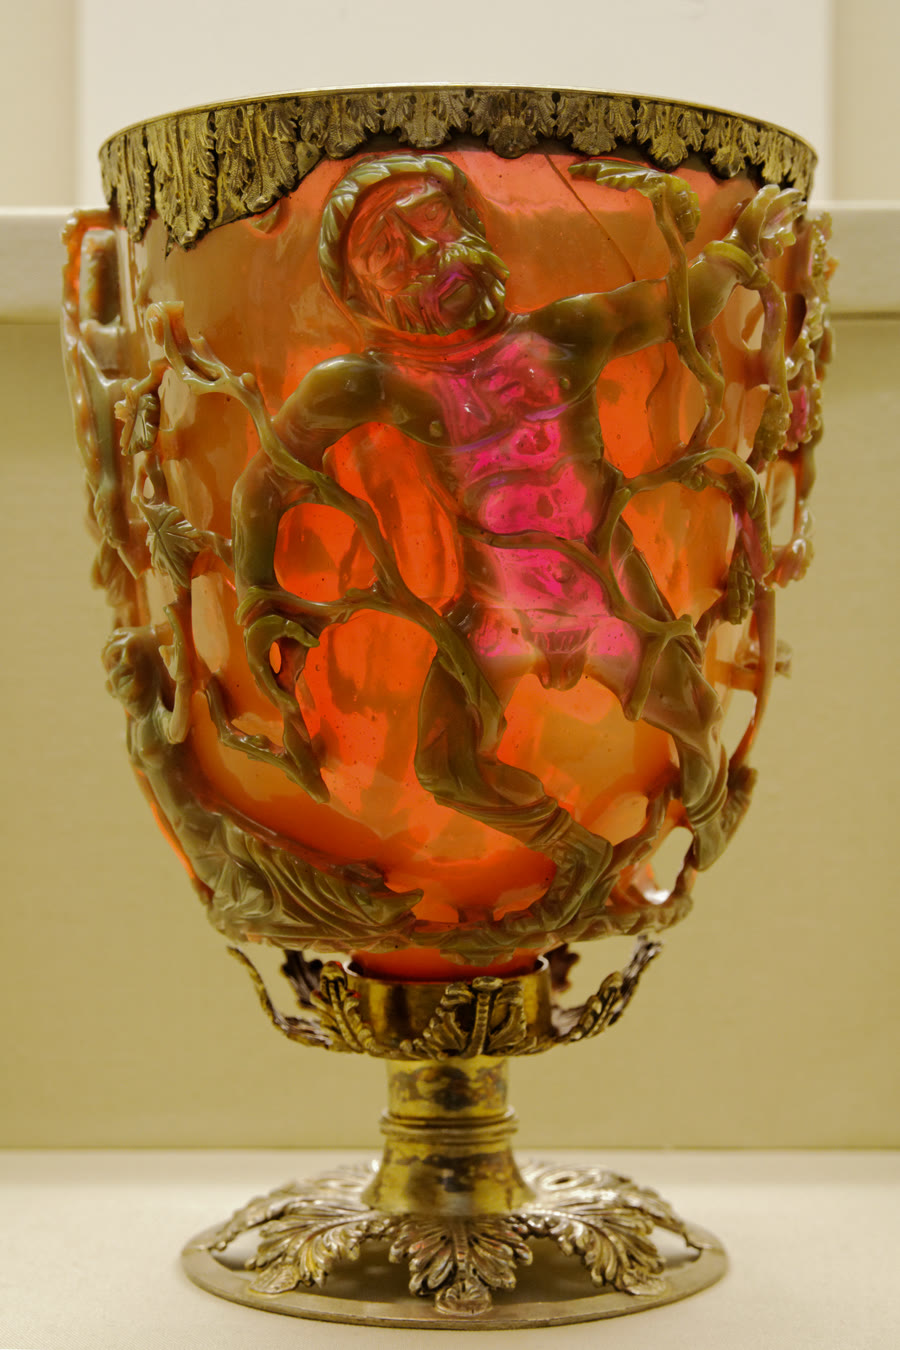
\includegraphics[width=0.32\linewidth]{images/book4/lycurgus-cup.jpg}

{\small A taça de Licurgo, um vidro romano do século IV, iluminada por dentro:
ela parece verde em luz refletida e vermelha em luz transmitida, um efeito de
\omterm{def:b3:inorganic-materials:nano}{nanopartículas} de ouro--prata no vidro. Fotografia: Marie-Lan Nguyen, CC BY
2.5.}
\end{omfigure}

\begin{history}[Nanopartículas antes da palavra, e uma bola de futebol de carbono]
Os vidreiros coloriam o vidro de vermelho com ouro muito antes de alguém saber por quê; a
taça de Licurgo mostra o efeito em sua forma mais marcante. Michael Faraday preparou \omterm{def:b3:colloids:colloid}{coloides}
de ouro na década de 1850 e viu que sua cor vinha de partículas pequenas demais
para serem vistas. Em 1985, Harold Kroto, Robert Curl e Richard Smalley, vaporizando
grafite com um laser, descobriram que aglomerados de sessenta átomos de carbono eram
excepcionalmente estáveis e propuseram a gaiola fechada de doze pentágonos e
vinte hexágonos; receberam o Prêmio Nobel de Química de 1996.
\end{history}

\section{Exercícios}

\begin{exercise}[$\star$]\label{exo:b3:inorganic-materials:1}
Uma camada de produto entre dois sólidos tem \qty{2.0}{\micro\metre} de espessura após \qty{10}{h}. Quanto tempo até
ela ter \qty{6.0}{\micro\metre} de espessura, se o crescimento for parabólico?
\end{exercise}

\begin{exercise}[$\star$]\label{exo:b3:inorganic-materials:2}
Escreva a hidrólise do ortossilicato de tetraetila em ácido silícico, a
condensação de duas moléculas de ácido silícico e a reação global que dá
sílica.
\end{exercise}

\begin{exercise}[$\star$]\label{exo:b3:inorganic-materials:3}
Classifique $\ce{SiO2}$, $\ce{B2O3}$, $\ce{Na2O}$ e $\ce{CaO}$ como formadores ou \omterm{def:b3:inorganic-materials:glass}{modificadores de rede}, e diga o que
$\ce{Na2O}$ faz com a rede da sílica.
\end{exercise}

\begin{exercise}[$\star$]\label{exo:b3:inorganic-materials:4}
Quantos pentágonos e hexágonos tem o $\ce{C70}$? Quantas ligações?
\end{exercise}

\begin{exercise}[$\star\star$]\label{exo:b3:inorganic-materials:5}
% ledger: rion:Sr2+XII, rion:Ca2+XII, rion:Ba2+XII, rion:Ti4+VI, rion:O2-VI
Calcule os \omterm{def:b3:inorganic-materials:perovskite}{fatores de tolerância} de $\ce{SrTiO3}$, $\ce{BaTiO3}$ e $\ce{CaTiO3}$ com os raios de coordenação doze
de $\ce{Sr^2+}$ (\qty{144}{pm}), $\ce{Ba^2+}$ (\qty{161}{pm}) e $\ce{Ca^2+}$ (\qty{134}{pm}), $r(\ce{Ti^4+}) = \qty{60.5}{pm}$ e $r(\ce{O^2-}) = \qty{140}{pm}$. O que
eles preveem?
\end{exercise}

\begin{exercise}[$\star\star$]\label{exo:b3:inorganic-materials:6}
Uma \omterm{def:b3:inorganic-materials:zeolite}{zeólita} X tem a fórmula anidra $\mathrm{Na_{86}[(AlO_2)_{86}(SiO_2)_{106}]}$ (dados do exercício).
Dê Si/Al e sua capacidade de troca para $\ce{Ca^2+}$ em milimols por grama.
\end{exercise}

\begin{exercise}[$\star\star$]\label{exo:b3:inorganic-materials:7}
% ledger: lat:Au
O ouro é cúbico de faces centradas com $a = \qty{407.8}{pm}$. Estime o número de camadas de uma
partícula cuboctaédrica de ouro de cerca de \qty{5}{nm} de diâmetro, seu número de átomos e a
fração deles na superfície.
\end{exercise}

\begin{exercise}[$\star\star$]\label{exo:b3:inorganic-materials:8}
Um \omterm{def:b3:solid-state:classes}{semicondutor} tem uma \omterm{def:b3:solid-state:band}{banda proibida}, no sólido maciço, de \qty{1.74}{eV}, e seu elétron e seu \omterm{def:b3:solid-state:carriers}{buraco}, uma \omterm{def:b3:quantum-model-systems:oscillator}{massa
reduzida} de $0.10\,m_e$ (dados do exercício). Estime a cor da luz emitida por
\omterm{def:b3:inorganic-materials:quantum-dot}{pontos quânticos} de raio 2.0 e \qty{3.0}{nm}, desprezando a atração coulombiana.
\end{exercise}

\begin{exercise}[$\star\star$]\label{exo:b3:inorganic-materials:9}
Os nanotubos $(10, 10)$, $(10, 0)$, $(9, 0)$ e $(12, 8)$ são metálicos ou \omterm{def:b3:solid-state:classes}{semicondutores}? Quais
são poltrona, quais zigue-zague?
\end{exercise}

\begin{exercise}[$\star\star\star$]\label{exo:b3:inorganic-materials:10}
% ledger: cod:MOF5.formula, cod:MOF5.a, cod:MOF5.Z
O MOF-5, $\mathrm{Zn_4O(C_8H_4O_4)_3}$, é cúbico com $a = \qty{25.82}{\angstrom}$ e oito unidades de fórmula por cela.
Calcule sua densidade. Se um grama tem uma área superficial de $\qty{3000}{m^2}$ (dados do
exercício), a quantos campos de futebol de $\qty{105}{m} \times \qty{68}{m}$ isso corresponde?
\end{exercise}

\begin{exercise}[$\star\star\star$]\label{exo:b3:inorganic-materials:11}
Usando a contagem de camadas da \cref{prop:b3:inorganic-materials:magic}, mostre que a
fração de superfície de um aglomerado cuboctaédrico tende a $3/n$ para $n$ grande, e
compare com a fração exata para $n = 8$.
\end{exercise}

\begin{exercise}[$\star\star\star$]\label{exo:b3:inorganic-materials:12}
Uma gaiola de carbono fechada, com três ligações por átomo, contém $p$ pentágonos, $h$ hexágonos
e $s$ heptágonos. Mostre que $p - s = 12$.
\end{exercise}

\section{Problema: Abrandar a água com a zeólita A}

\begin{problem}[{Problema de fim de semana --- abrandar a água com a zeólita A: a
fórmula e a regra de Löwenstein, a capacidade de troca teórica, a zeólita
necessária para uma lavagem e a janela que deixa entrar o cálcio e mantém os detergentes
do lado de fora}]
\label{pb:b3:inorganic-materials:1}
% ledger: iza:LTA.formula, iza:LTA.window, aw:Na, aw:Al, aw:Si, aw:O, aw:H, aw:Ca, aw:C, rion:Ca2+VI
A \omterm{def:b3:inorganic-materials:zeolite}{zeólita} A, usada nos detergentes no lugar dos fosfatos, tem a fórmula
$\mathrm{Na_{12}[(AlO_2)_{12}(SiO_2)_{12}]\cdot 27H_2O}$ e janelas de \qty{0.41}{nm}. Uma água de torneira contém
\qty{2.0}{mmol/L} de $\ce{Ca^2+}$, e uma lavagem usa \qty{15}{L} dela; no tempo de uma lavagem, a \omterm{def:b3:inorganic-materials:zeolite}{zeólita}
atinge 60\,\% de sua capacidade (dados do problema).

\medskip\noindent\textbf{Parte I --- A fórmula.}
\begin{enumerate}
  \item Calcule a massa molar da fórmula anidra.
  \item Calcule a da fórmula hidratada.
  \item Dê Si/Al.
  \item Enuncie a regra de Löwenstein e o que ela implica aqui para o arranjo de
        Si e Al.
  \item Qual é a carga da estrutura por fórmula?
  \item Calcule a fração mássica de água na \omterm{def:b3:inorganic-materials:zeolite}{zeólita} hidratada.
\end{enumerate}

\medskip\noindent\textbf{Parte II --- Capacidade de troca.}
\begin{enumerate}[resume]
  \item Escreva o equilíbrio de troca entre a \omterm{def:b3:inorganic-materials:zeolite}{zeólita} sódica e os íons
        cálcio.
  \item Quantos $\ce{Ca^2+}$ uma fórmula pode captar?
  \item Calcule a capacidade teórica da \omterm{def:b3:inorganic-materials:zeolite}{zeólita} anidra em mmol de $\ce{Ca^2+}$
        por grama.
  \item Calcule-a para a \omterm{def:b3:inorganic-materials:zeolite}{zeólita} hidratada.
  \item Exprima a capacidade anidra em miligramas de $\ce{CaCO3}$ por grama, a unidade usual
        da dureza da água.
\end{enumerate}

\medskip\noindent\textbf{Parte III --- Uma lavagem.}
\begin{enumerate}[resume]
  \item Calcule a quantidade de $\ce{Ca^2+}$ na água de uma lavagem.
  \item Calcule a massa de \omterm{def:b3:inorganic-materials:zeolite}{zeólita} hidratada necessária na capacidade teórica.
  \item Calcule-a a 60\,\% da capacidade.
  \item Calcule a massa de sódio liberada na água.
  \item Por que os fabricantes de detergentes substituíram os fosfatos?
  \item Por que a \omterm{def:b3:inorganic-materials:zeolite}{zeólita} A capta $\ce{Mg^2+}$ mais lentamente que $\ce{Ca^2+}$?
\end{enumerate}

\medskip\noindent\textbf{Parte IV --- A janela.}
\begin{enumerate}[resume]
  \item Compare a janela com o diâmetro de um íon $\ce{Ca^2+}$ (raio de coordenação seis
        \qty{100}{pm}).
  \item O que um íon $\ce{Ca^2+}$ hidratado precisa fazer para passar?
  \item Por que um ânion \omterm{def:b3:colloids:surfactant}{tensoativo} como o dodecilsulfato fica de fora?
  \item O que a \omterm{def:b3:inorganic-materials:zeolite}{zeólita} A faz como agente secante, e por que ela é chamada de
        \omterm{def:b3:inorganic-materials:zeolite}{peneira molecular}?
  \item Como a substituição de $\ce{Na+}$ por $\ce{K+}$ alteraria o tamanho das moléculas admitidas?
  \item Na ZSM-5, por que o \textit{para}-xileno sai dos poros mais depressa que o \textit{orto}-xileno?
  \item Enuncie o resultado: a capacidade de troca teórica da \omterm{def:b3:inorganic-materials:zeolite}{zeólita} A anidra
        para $\ce{Ca^2+}$.
\end{enumerate}
\end{problem}
